

\section{Introduction}

%From Wikipedia, the free encyclopedia.
%
%In probability theory and statistics, a Gaussian process is a particular kind of statistical model where observations occur in a continuous domain, \eg time or space. In a Gaussian process, every point in some continuous input space is associated with a normally distributed random variable. Moreover, every finite collection of those random variables has a multivariate normal distribution, i.e. every finite linear combination of them is normally distributed. The distribution of a Gaussian process is the joint distribution of all those (infinitely many) random variables, and as such, it is a distribution over functions with a continuous domain, e.g. time or space. 
%
%
%Viewed as a machine learning algorithm, a Gaussian process uses lazy learning and a measure of the similarity between points (the kernel function) to predict the value for an unseen point from training data. The prediction is not just an estimate for that point, but also has uncertainty information it is a one-dimensional Gaussian distribution (which is the marginal distribution at that point).
%
%For some kernel functions, matrix algebra can be used to calculate the predictions using the technique of Kriging. When a parameterized kernel is used, optimization software is typically used to fit a Gaussian process model.
%
%The concept of Gaussian processes is named after Carl Friedrich Gauss because it is based on the notion of the Gaussian distribution (normal distribution). Gaussian processes can be seen as an infinite-dimensional generalization of multivariate normal distributions.
%
%Gaussian processes are useful in statistical modeling, benefiting from properties inherited from the normal. For example, if a random process is modeled as a Gaussian process, the distributions of various derived quantities can be obtained explicitly. Such quantities include the average value of the process over a range of times and the error in estimating the average using sample values at a small set of times.

A Hilbert space is a real or complex inner product space with respect to the distance function induced by the inner product \cite{dieudonne2013foundations}. Particularly, the Hilbert space $\mathcal{L}_2[0,1]$ is a set of square integrable functions $f(t):[0,1]\rightarrow\mathbb{R}$, where all functions satisfy 
\begin{equation*}
\mathcal{L}_2[0,1] =\lbrace f:\int_0^1f^2dt <\infty \rbrace
\end{equation*}
with an inner product $\langle f,g\rangle=\int_0^1fgdt$. 

Consider a regression problem with observations $y_i = f(t_i)+\varepsilon_i$, $i=1,\ldots,n$, consisting \iid normal noises $\varepsilon_i\sim N(0,\sigma^2)$ in the space $C^{(m)}[0,1]=\{ f:f^{(m)}\in \mathit{L}_2[0,1] \}$. The classic nonparametric or semi-parametric regression is a function that minimizes the following penalized least square functional 
\begin{equation}\label{GaussianProcessGeneralObjective}
\frac{1}{n}\sum_{i=1}^{n}\left( y_i-f(t_i) \right)^2 + \lambda \int_{0}^{1} \left( f^{(m)}\right)^2dt, 
\end{equation}
where the first term is the lack of fit of $f$ to the data. In the second term, generally, $\lambda$ is a fixed smoothing parameter controlling the trade-off between over-fitting and bias \cite{esl2009}. The minimizer $f_\lambda$ of the above equation resides in an $n$-dimensional space and the computation in multivariate settings is generally of the order $O(n^3)$ \cite{kim2004smoothing}. It is shown that a piecewise polynomial smoothing spline of degree $2m-1$ is well known to provide an aesthetically satisfying method for estimating $f$ if $\mathbf{y}$ cannot be interpolated exactly by some polynomial of degree less than $m$ \cite{schoenberg1964spline}. For instance, when $m=2$, a piecewise cubic smoothing spline provides a powerful tool to estimate the above nonparametric function, in which the penalty term is $\int f''^2dt$ \cite{hastie1990generalized}. 



Further, \cite{wahba1978improper} showed that a Bayesian version of this problem is to take a Gaussian process prior $f(t_i) = a_0+a_1t_i+\cdots + a_{m-1}t_i^{m-1} + x_i$, on $f$ with $x_i=X(t_i)$ being a zero mean Gaussian process whose $m$th derivative is scaled white noise, $i=1,\ldots,n$ \cite{speckman2003fully}. The extended Bayes estimates $f_\lambda$ with a "partially diffuse" prior is as exactly the same as spline solution. Some works have been done on discovering the relationship between nonparametric regression and Bayesian estimation. \cite{heckman1991minimax} shows that if $f$ the regression function $\E(y\mid f)$ has unknown prior distribution  $\mathbf{f}=(f(t_1),\ldots,f(t_n))^\top$ lying in a known class of $\Omega$, then the maximum is taken over all priors in $\Omega$ and the minimum is taken over linear estimator of $\mathbf{f}$. \cite{branson2017nonparametric} propose a Gaussian process regression method that acts as a Bayesian analog to local linear regression for sharp regression discontinuity designs. It is no doubt that one of the attractive features of the Bayesian approach is that, in principle, one can solve virtually any statistical decision or inference problem. Particularly, one can provide an accuracy assessment for $\hat{f}=\E (f\mid \mathbf{y})$ using posterior probability regions \cite{cox1993analysis}. 


Based on the correspondence, \cite{craven1978smoothing} proposed an generalized cross-validation estimate for the minimizer $f_\lambda$. The estimate $\hat{\lambda}$ is the minimizer of the function where the trace of matrix $A(\lambda)$ in (\ref{crossvalidationmatrixA}) is incorporated. It is also able to establish an optimal convergence property for their estimator when the number of observations in a fixed interval tends to infinity \cite{wecker1983signal}. A high efficient  algorithm to optimize generalized cross-validation and generalized maximum likelihood scores with multiple smoothing parameters via the newton method was proposed by \cite{gu1991minimizing}. This algorithm can also be applied to the maximum likelihood and the restricted maximum  likelihood estimation. The behavior of the optimal regularization parameter in the method of regularization was investigated by \cite{wahba1990optimal}. 



In this chapter, we prove that the Tractor spline can be estimated by Bayesian approach in second-derivative-piecewise-continuous Reproducing Kernel Hilbert Space. The GCV is used to find the optimal parameters for Tractor spline. 



\section{Polynomial Smoothing Splines on $[0, 1]$ as Bayes Estimates}

A polynomial smoothing spline of degree $2m-1$ is a piecewise polynomial of the same degree in each intervals $[t_i,t_{i+1}]$, $i=1, \ldots, n-1$, and the first $2m-2$ derivatives are continuous at joint knots. For instance, when $m=2$,  a piecewise cubic smoothing spline is a special case of the polynomial smoothing spline providing a powerful tool to estimate the above nonparametric function (\ref{GaussianProcessGeneralObjective}) in the space  $\mathcal{C}^{(2)}[0,1]$, where the penalty term is $\int f''^2dt$ \cite{hastie1990generalized}  \cite{wang1998smoothing}. If a general space $\mathcal{C}^{(m)}[0,1]$ is equipped with an appropriate inner product, it can be made a reproducing kernel Hilbert space. 

\subsection{Polynomial Smoothing Spline}

A spline is a numeric function that is piecewise-defined by polynomial functions, and which possesses a high degree of smoothness at the places where the polynomial pieces connect (known as knots) \cite{judd1998numerical} \cite{chen2009feedback}. Suppose we are given observed data $(t_1,y_1),(t_2,y_2), \ldots, (t_n,y_n)$ in interval $[0,1]$, satisfying $0\leq t_1< t_2 < \cdots <t_n \leq 1$, a piecewise polynomial function $f(t)$ can be obtained by dividing the interval into contiguous intervals $(t_1,t_2),\ldots,(t_{n-1},t_n)$ and represented by a separate polynomial in each interval. For any continuous $f\in \mathcal{C}^{(m)}[0,1]$, it can be represented in a linear combination of basis functions $h_m(t)$ as $f(t) =\sum_{m=1}^{M}\beta_mh_m(t)$, where $\beta_m$ are coefficients \cite{ellis2009}. It is just like every vector in a vector space can be represented as a linear combination of basis vectors. 



A smoothing polynomial spline is uniquely the smoothest function that achieves a given degree of fidelity to a particular data set \cite{whittaker1922new}. In deed, the minimizer of function (\ref{GaussianProcessGeneralObjective}) is the curve estimate $\hat{f}(t)$ over all spline functions $f(t)$ with $m-1$ continuous derivatives fitting observed data in the space $\mathcal{C}^{(m)}[0,1]$. In fact, \cite{kimeldorf1971some},  \cite{kimeldorf1970correspondence}  prove that the minimizer $f_\lambda$ of function (\ref{GaussianProcessGeneralObjective}) has the form 
\begin{equation}
f(t)=\sum_{\nu=1}^m d_\nu \phi_\nu(t)+\sum_{i=1}^n c_iR_1(t,t_i).
\end{equation}
%where $\phi_\nu (t)=\frac{t^{\nu-1}}{(\nu-1)!}$, $\nu=1, \ldots, m$. 
where $\{\phi_\nu(t)\}$ is a set of basis functions of space $\mathcal{H}_0$ and $R(\cdot,\cdot)$ is the reproducing kernel in $\mathcal{H}_1$. 



\subsection{Reproducing Kernel Hilbert Space $\mathcal{H}^{(m)}[0,1]$}

For any $f\in \mathcal{C}^{(m)}[0,1]$, its standard Taylor expansion is  
\begin{equation}
f(t) = \sum_{\nu=0}^{m-1}\frac{t^\nu}{\nu!}f^{(\nu)}(0) + \int_{0}^{1}\frac{(t-u)_+^{m-1}}{(m-1)!}f^{(m)}(t)dt,
\end{equation}
where $(\cdot)_+ =\max(0, \cdot)$. With an inner product 
\begin{equation}
\langle f,g \rangle = \sum_{\nu=0}^{m-1}f^{(\nu)}(0)g^{(\nu)}(0) +  \int_{0}^{1}f^{(m)} g^{(m)}dt,
\end{equation}
the representer is 
\begin{equation}\label{GaussianProcessKernelR}
R_s(t) =\sum_{\nu=0}^{m-1} \frac{s^{\nu}}{\nu!} \frac{t^{\nu}}{\nu!} +\int_0^1\frac{ (s-u)_+^{m-1}}{(m-1)!} \frac{ (t-u)_+^{m-1}}{(m-1)!} du \triangleq R_0(s,t)+R_1(s,t). 
\end{equation}
It is easily to prove that $R(s,t)$ is non-negative and is reproducing kernel, by which $\langle R(s,t),f(t) \rangle = \langle R_s(t),f(t) \rangle=f(s)$. Additionally, $R_s^{(\nu)}(0) = s^\nu/\nu!$ for $\nu = 0,\ldots, m-1$.

Before moving on to further steps, we are now introducing the following two theorems. 
\begin{theorem}\cite{aronszajn1950theory}\label{theoremRKHS}
Suppose $R$ is a symmetric, positive definite kernel on a set $X$. Then there is a unique Hilbert space of functions on $X$ for which $R$ is a reproducing kernel. 
\end{theorem}
\begin{theorem}\cite{gu2013smoothing}\label{theoremKernel}
If the reproducing kernel $R$ of a space $\mathcal{H}$ on domain $X$ can
be decomposed into $R = R_0 + R_1$, where $R_0$ and $R_1$ are both non-negative definite, $R_0(x, \cdot),R1(x,\cdot) \in \mathcal{H}$, for $ \forall x \in X$, and $\langle R_0(x, \cdot),R_1(y, \cdot) \rangle= 0$, for $\forall x, y \in X$, then the spaces $\mathcal{H}_0$ and $\mathcal{H}_1$ corresponding respectively to $R_0$ and $R_1$ form a tensor sum decomposition of $\mathcal{H}$. Conversely, if $R_0$ and $R_1$ are both  nonnegative definite and $\mathcal{H}_0 \cap \mathcal{H}_1 =\{0\}$, then $\mathcal{H} =\mathcal{H}_0 \oplus \mathcal{H}_1$ has a reproducing kernel $R = R_0 + R_1$.
\end{theorem}

According to theorem \ref{theoremRKHS}, the Hilbert space associated with $R$ can be constructed as containing all finite linear combinations of the form $\sum a_iR(t_i,\cdot)$, and their limits under the norm induced by the inner product $\langle R(s,\cdot),R(t,\cdot) \rangle = R(s,t)$. As for theorem \ref{theoremKernel}, it is easy to verify that $R_0$ corresponds to the space of polynomials $\mathcal{H}_0 =\{f:f^{(m)}=0\}$ with an inner product $\langle f, g \rangle_0 = \sum_{\nu=0}^{m-1} f^{(\nu)}(0)g^{(\nu)}(0)$ and $R_1$ corresponds to the orthogonal complement of $\mathcal{H}_0$, that is $\mathcal{H}_1 =\{  f:f^{(\nu)}(0)=0,\nu = 0, \ldots,m-1, \int_{0}^{1}(f^{(m)})^2dt <\infty  \}$ with an inner product $\langle f, g\rangle_1 = \int_{0}^{1}f^{(m)}g^{(m)}dt $. 






\subsection{Polynomial Smoothing Spline as Bayes Estimates}

Because it is possible to interpret the smoothing spline regression estimator as a Bayes estimate when the mean function $r(\cdot)$ is given an improper prior distribution \cite{wahba1990spline} \cite{berlinet2011reproducing}, therefore, we will find that the posterior mean of $f=f_0+f_1$ on $[0,1]$ with proper priors is the polynomial smoothing  spline of (\ref{GaussianProcessGeneralObjective}). 

Indeed, we can find out every $f=f_0+f_1$ on $[0,1]$ with $f_0$ and $f_1$ having independent Gaussian priors with zero means and covariances as 
\begin{align*}
\E (f_0(s)f_0(t)) &= \tau^2 R_0(s,t)=\tau^2 \sum_{\nu=0}^{m-1}\frac{s^\nu}{\nu!}\frac{t^\nu}{\nu!}, \\
\E (f_1(s)f_1(t)) &= bR_1(s,t) = b\int_{0}^{1} \frac{(s-u)_+^{m-1}}{(m-1)!} \frac{(t-u)_+^{m-1}}{(m-1)!},
\end{align*}
where $R_0$ and $R_1$ are from (\ref{GaussianProcessKernelR}). Because of the observations are normally distributed as $y_i\sim N(f(t_i),\sigma^2)$, then the joint distribution for $\mathbf{y} = \{y_1,\ldots,y_n\}$ and $f(t)$ is normal with zero mean and the following covariance matrix 
\begin{align*}\Cov (\mathbf{f},\mathbf{y}) = 
\begin{bmatrix}
bQ+\tau SS^\top+\sigma^2 I & b\xi +\tau^2 S\phi \\
b\xi^\top + \tau^2\phi^\top S^\top & bR_1(t,t) +\tau^2\phi^\top \phi
\end{bmatrix},
\end{align*}
where $\{Q_{i,j}\}_{n\times n}=R_1(t_i,t_j)$, $\{S_{i,\nu}\}_{n\times m}=t_i^{\nu-1}/(\nu-1)!$, $\{\xi_{i,1}\}_{n\times 1}=R_1(t_i,t)$ and $\{\phi_{\nu,1}\}_{m\times 1}=t^{\nu-1}/(\nu-1)!$. 
Consequently, the posterior is 
\begin{equation}
\begin{split}
\E (f(t)\mid\mathbf{y}) &= (b\xi^\top +\tau \phi^\top s^\top)(bQ+\tau^2 SS^\top+\sigma^2I)^{-1}\mathbf{y} \\
&= \xi^\top(Q+\rho SS^\top+n\lambda I)^{-1}\mathbf{y}+ \phi^\top\rho S^\top(Q+\rho SS^\top +n\lambda I)^{-1}\mathbf{y},
\end{split}
\end{equation}
where $\rho = \tau^2/b$ and $n\lambda=\sigma^2/b$. Furthermore, by denoting $M=Q+n\lambda I$, \cite{gu2013smoothing} gives that, when $\rho\rightarrow \infty$, the posterior mean is in the form $\E(f(t)\mid y_{1:n}) = \xi^\top\mathbf{c}+\phi^\top\mathbf{d}$ with coefficients
\begin{align}
\mathbf{c}&=(M^{-1}-M^{-1}S(S^\top M^{-1}S)^{-1}S^\top M^{-1})\mathbf{y},\\
\mathbf{d}&=(S^\top M^{-1}S)^{-1}S^\top M^{-1}\mathbf{y}.
\end{align}

\begin{theorem}\cite{gu2013smoothing}
The polynomial smoothing spline of (\ref{GaussianProcessGeneralObjective}) is the posterior mean of $f = f_0 +f_1$, where $f_0$ diffuses in span $\{t^{\nu-1}, \nu= 1, \ldots , m\}$ and $f_1$ has a Gaussian process prior with mean zero and a covariance function
\begin{equation*}
bR_1(s,t) = b\int_{0}^{1} \frac{(s-u)_+^{m-1}}{(m-1)!} \frac{(t-u)_+^{m-1}}{(m-1)!},
\end{equation*}
for $b=\sigma^2/n\lambda$. 
\end{theorem}



\subsection{Gaussian Process Regression}

Gaussian processes are the extension of multivariate Gaussian to infinite-sized collections of real value variables, any finite number of which have a joint Gaussian distribution \cite{rasmussen2006gaussian}. Gaussian process regression is a probability distribution over functions. It is fully defined by its mean $m(t)$ and covariance $K(s,t)$ function as 
\begin{align*}
m(t)&=\E [f(t)] \\
K(s,t)&=\E \lbrack (f(s)-m(s)) (f(t)-m(t))\rbrack,
\end{align*}
where $s$ and $t$ are two variables. A function $f$ distributed as such is denoted in form of 
\begin{equation*}
f \sim GP(m(t),K(s,t)).
\end{equation*}
Usually the mean function is assumed to be zero everywhere. 

Given a set of input variables $\mathbf{t} = \{t_1,\ldots,t_n\}$ for function $f(t)$ and the output $\mathbf{y}=f(\mathbf{t})+\varepsilon$ with independent identically distributed Gaussian noise $\varepsilon$ with variance $\sigma_n^2$,  we can use the above definition to predict the value of the function $f_*=f(t_*)$ at a particular input $t_*$. As the noisy observations becoming
\begin{equation*} %\label{GaussianProcessCovDef}
\Cov (y_p,y_q) = K(t_p,t_q)+\sigma_n^2 \delta_{pq}
\end{equation*}
where $\delta_{pq}$ is a Kronecker delta which is one if and only if $p=q$ and zero otherwise, the joint distribution of the observed outputs $\mathbf{y}$ and the estimated output $f_*$ according to prior is
\begin{equation}
\begin{bmatrix}
\mathbf{y}\\
f_*
\end{bmatrix} \sim N \left(  
0,  \begin{bmatrix}
K(\mathbf{t},\mathbf{t}) +\sigma_n^2I& K(\mathbf{t},t_*) \\
K(t_*,\mathbf{t}) & K(t_*,t_*)
\end{bmatrix} 
\right).
\end{equation}
The posterior distribution over the predicted value is obtained by conditioning on the observed data
\begin{equation*}
f_* \mid  \mathbf{y},\mathbf{t},t_* \sim N(\bar{f_*},\Cov (f_*))
\end{equation*}
where 
\begin{align}
\bar{f_*}&=\E [f_* \mid  \mathbf{y},\mathbf{t},t_* ]=K(t_*,\mathbf{t})[K(\mathbf{t},\mathbf{t})+\sigma_n^2I]^{-1}\mathbf{y},\\
\Cov(f_*)&=K(t_*,t_*)-K(t_*,\mathbf{t})[K(\mathbf{t},\mathbf{t})+\sigma_n^2I]^{-1}K(\mathbf{t},t_*).
\end{align}
Therefore, we can see that the Bayesian estimation of smoothing spline is a special format of Gaussian process regression with diffuse prior and the covariance matrix $R(s,t)$. 





\section{Tractor Spline as Bayes Estimate}


Recall the definition of Tractor spline introduced in Chapter \ref{SectionTractorSpline}. It is the solution to the objective function (\ref{tractorsplineObjective}), where an extra term for $f'(t)-v$ and an extra parameter $\gamma$ are incorporated. The penalty parameter $\lambda(t)$ is a function varying on different domains. If $\lambda(t)=\lambda$ is constant and $\gamma=0$, the Tractor spline degenerate to a conventional cubic smoothing spline consisting of a set of given basis functions.  

However, the Bayes estimate for a polynomial smoothing spline requires fixed interval on $[0,1]$ and the penalty parameter being constant. For the first constraint, with generality, an arbitrary interval $[a,b]$ can be transformed to $[0,1]$. For the second constraint, we assume that $\lambda(t)$ stays the same constant on each subinterval of $[0,1]$ and name the solution "trivial Tractor spline".  In this section, I still call it the "Tractor spline" for sake of simplicity. 


In the following, we are going to prove that this kind of trivial Tractor spline is corresponding to Bayes estimate in a particular reproducing kernel Hilbert space. 


\subsection{Reproducing Kernel Hilbert Space $\mathcal{C}_{\footnotesize p.w.}^{2}[0,1]$}

The space $C^{(m)}[0,1]=\{ f:f^{(m)}\in \mathit{L}_2[0,1] \}$ is a set of functions $f$ whose $m$th derivatives are square integrable on the domain $[0,1]$. For a tractor spline, it only requires $m=2$. In fact, its second derivative is piecewise linear but is not necessarily continuous at joint knots. Besides, only if $\lambda(t)$ is constant and $\gamma=0$, the second derivative is piecewise linear and continuous at joint knots. Here we are introducing the space 
\begin{equation*}
\mathcal{C}_{\footnotesize p.w.}^{2}[0,1]=\{f: f''\in \mathit{L}_2[0,1], f,f' \mbox{ are continuous and } f'' \mbox{ is piecewise linear}\},
\end{equation*}
in which the second derivative of any function $f$ is not necessarily continuous. 


Given a sequence of paired data $\{(t_1,y_1,v_1),\ldots, (t_n,y_n,v_n) \}$, the the minimizer of 
\begin{equation}\label{maineq}
\frac{1}{n}\sum_{i=1}^{n}(y_i-f(t_i))^2+\frac{\gamma}{n}\sum_{i=1}^{n}(v_i-f'(t_i))^2+\lambda \int_{0}^{1}f''^2dt
\end{equation}
in the space $\mathcal{C}_{\footnotesize p.w.}^{2}[0,1]$ is a Tractor spline. Equipped with an appropriate inner product
\begin{equation}\label{TractorSplineInnerProduct}
\langle f,g \rangle=f(0) g(0)+f'(0) g'(0)+\int_{0}^{1}f''g''dx,
\end{equation}
the space $\mathcal{C}_{\footnotesize p.w.}^{2}[0,1]$ is made a reproducing kernel Hilbert space. In fact, the representer $R_s(\cdot)$ is 
\begin{equation}\label{kerneleq}
R_s(t)=1+st+\int_{0}^{1} (s-u)_+(t-u)_+du.
\end{equation}
It can be seen that $R_s(0)=1, R'_s(0)=s$, and $R''_s(t)=(s-t)_+$. The two terms of the reproducing kernel $R(s,t)=R_s(t)\triangleq R_0(s,t)+R_1(s,t)$, where
\begin{align*} %\label{TractorSplineKernelR0}
R_0(s,t)&=1+st \\ %\label{TractorSplineKernelR1}
R_1(s,t)&=\int_{0}^{1} (s-u)_+(t-u)_+du
\end{align*}
are both non-negative definite themselves.


According to Theorem \ref{theoremKernel}, $R_0$ can correspond the space of polynomials $\mathcal{H}_0=\{f:f''=0\}$ with an inner product $\langle f,g \rangle_0= f(0)g(0)+f'(0)g'(0)$, and $R_1$ corresponds the orthogonal complement of $\mathcal{H}_0$
\begin{equation*}
\mathcal{H}_1=\{f:f(0)=0, f'(0)=0, \int_{0}^{1}f''^2dt<\infty\}
\end{equation*}
with inner product $\langle f,g \rangle_1=\int_{0}^{1}f''g''dt$. Thus, $\mathcal{H}_0$ and $\mathcal{H}_1$ are two subspaces of the $\mathcal{C}_{\footnotesize p.w.}^{2}[0,1]$, and the reproducing kernel is $R_s(\cdot) = R_0(s,\cdot)+R_1(s,\cdot)$.


Define a new notation $\dot{R}(s,t)=\frac{\partial R}{\partial s}(s,t)=\frac{\partial R_0}{\partial s}(s,t)+\frac{\partial R_1}{\partial s}(s,t)=t+\int_0^s(t-u)_+du$. Obviously $\dot{R}_s(t) \in \mathcal{C}_{\footnotesize p.w.}^{2}[0,1]$. Additionally, we have $\dot{R}_s(0)=0, \dot{R}'_s(0)=\frac{\partial \dot{R}_s}{\partial t}(0)=1$, and $ \dot{R}''_s(t)=\begin{cases}
0 & s\leq t \\ 1 & s>t \end{cases}$. Then, for any $f\in \mathcal{C}_{\footnotesize p.w.}^{2}[0,1]$, we have 
\begin{equation*}
\langle \dot{R}_s,f\rangle =\dot{R}_s(0)f(0)+\dot{R}'_s(0)f'(0)+\int_0^1\dot{R}''_s f''	 du=f'(0)+\int_0^t f''du=f'(t).
\end{equation*}
% % % % % % % % % % % % % % % %  Old version, space H* might be wrong % % % % %
% % % % % % % % % % % % % % % %
%It can be seen that the first term $\dot{R}_0=t\in \mathcal{H}_0$, and the space spanned by the second term $\dot{R}_1=\int_0^s(t-u)_+du$, denoted as $\mathcal{\dot{H}}$, is not in $\mathcal{H}_1$, but $\mathcal{\dot{H}} \cap \mathcal{H}_1\neq \emptyset$. Then we have a new space $\mathcal{H}_*=\mathcal{\dot{H}} \cup \mathcal{H}_1$. Thus the two new sub spaces in $\mathcal{C}_{\footnotesize p.w.}^2[0,1]$ are $\mathcal{H}_0$ and $\mathcal{H}_*$.
%
%Given the sample points $t_j, j=1, \ldots, n$ in equation $(\ref{maineq})$ and noting that the space
%\begin{equation}
%\mathcal{A}=\{f: f=\sum_{j=1}^{n}\alpha_jR_1(t_j,\cdot)+\sum_{j=1}^{n}\beta_j\dot{R}_1(t_j,\cdot)\} 
%\end{equation}
%is a closed linear subspace of $\mathcal{H}_*$. Then $f  \in \mathcal{C}_{\footnotesize p.w.}^2[0,1]$ can be written as
%\begin{equation}\label{GaussianProcessFunctionF}
%f(t)=d_1+d_2t+\sum_{j=1}^{n}c_jR_1(t_j,t)+\sum_{i=j}^{n}b_j\dot{R}_1(t_j,\cdot) +\rho(t)
%\end{equation}
%where $\mathbf{d},\mathbf{c}$ and $\mathbf{b}$ are coefficients, and $\rho(t) \in \mathcal{H}_* \ominus \mathcal{A}$. 
It can be seen that the first term $\dot{R}_0=t\in \mathcal{H}_0$, and the space spanned by the second term $\dot{R}_1=\int_0^s(t-u)_+du$, denoted as $\mathcal{\dot{H}}$, is a subspace of $\mathcal{H}_1$, and $\mathcal{\dot{H}} \ominus \mathcal{H}_1\neq \emptyset$. Given the sample points $t_j, j=1, \ldots, n$, in equation $(\ref{maineq})$ and noting that the space
\begin{equation*}
\mathcal{A}=\{f: f=\sum_{j=1}^{n}\alpha_jR_1(t_j,\cdot)+\sum_{j=1}^{n}\beta_j\dot{R}_1(t_j,\cdot)\} 
\end{equation*}
is a closed linear subspace of $\mathcal{H}_1$. Then we have a new space $\mathcal{H}_*=\mathcal{\dot{H}} \cup \mathcal{A}$. Thus the two new sub spaces in $\mathcal{C}_{\footnotesize p.w.}^2[0,1]$ are $\mathcal{H}_0$ and $\mathcal{H}_*$.


For any $f  \in \mathcal{C}_{\footnotesize p.w.}^2[0,1]$, it can be written as 
\begin{equation}\label{GaussianProcessFunctionF}
f(t)=d_1+d_2t+\sum_{j=1}^{n}c_jR_1(t_j,t)+\sum_{i=j}^{n}b_j\dot{R}_1(t_j,\cdot) +\rho(t)
\end{equation}
where $\mathbf{d},\mathbf{c}$ and $\mathbf{b}$ are coefficients, and $\rho(t) \in \mathcal{H}_1 \ominus \mathcal{H}_*$. Thus, by substituting to the equation $(\ref{maineq})$, it can be written as 
\begin{equation}\label{GassianProcessRawequation}
\begin{split}
&\frac{1}{n}\sum_{i=1}^n \left( y_i - d_1-d_2t-\sum_{j=1}^{n}c_jR_1(t_j,t_i)-\sum_{j=1}^{n}b_j\dot{R}_1(t_j,t_i)-\rho(t_i) \right) ^2\\
&\frac{\gamma}{n}\sum_{i=1}^n \left( v_i - d_2-\sum_{j=1}^{n}c_jR'_1(t_j,t_i)-\sum_{j=1}^{n}b_j\dot{R}'_1(t_j,t_i)-\rho'(t_i) \right) ^2\\
+&\lambda \int_0^1 \left( \sum_{j=1}^{n}c_jR''_1(t_j,t)+\sum_{j=1}^{n}b_j\dot{R}''_1(t_j,t)+\rho''(t)\right)^2dt
\end{split}
\end{equation}
Because of orthogonality, $\rho(t_i) = (R_1(t_i,\cdot),\rho)=0$, $\rho'(t_i) = (\dot{R}_1(t_i,\cdot),\rho')=0$, $i=1,\ldots,n$. By denoting that 
\begin{align*}
S&=\{S_{ij} \}_{n\times 2}=\begin{bmatrix}1 & t_i \end{bmatrix} ,& Q&=\{Q_{ij} \}_{n\times n}= R_1(t_j,t_i), & P&=\{P_{ij} \}_{n\times n}= \dot{R}_1(t_j,t_i), \\
S'&=\{S'_{ij} \}_{n\times 2}=\begin{bmatrix} 0 & 1 \end{bmatrix} ,& Q'&=\{Q'_{ij} \}_{n\times n}= R_1'(t_j,t_i), & P'&=\{P'_{ij} \}_{n\times n}= \dot{R}_1'(t_j,t_i). 
\end{align*}
and noting that $\int_0^1R''_1(t_i,t)R''_1(t_j,t)dt=R_1(t_i,t_j)$, $\int_0^1R''_1(t_i,t)\dot{R}''_1(t_j,t)dt=\int_0^{v}(t_i-t)dt=\dot{R}_1(t_j,t_i)$, and $\int_0^1\dot{R}''_1(t_i,t)\dot{R}''_1(t_j,t)dt=\int_0^{v}1dt=\dot{R}'_1(t_i,t_j)$, where $v=\mbox{min}(t_i,t_j)$, the above equation (\ref{GassianProcessRawequation}) can be written as 
\begin{equation}\label{matriteq}
\begin{split}
(\mathbf{y}-S\mathbf{d}-Q\mathbf{c}-P\mathbf{b})^\top (\mathbf{y}-S\mathbf{d}-Q\mathbf{c}-P\mathbf{b})+\\
\gamma(\mathbf{v}-S'\mathbf{d}-Q'\mathbf{c}-P'\mathbf{b})^\top (\mathbf{v}-S'\mathbf{d}-Q'\mathbf{c}-P'\mathbf{b})\\
+n\lambda (\mathbf{c}^\top Q\mathbf{c} + 2\mathbf{c}^\top P\mathbf{b}+ \mathbf{b}^\top P'\mathbf{b})+n\lambda(\rho,\rho).
\end{split}
\end{equation}
Note that $\rho$ only appears in the third term and is minimized at $\rho=0$. Hence, a tractor spline resides in the space $\mathcal{H}_0\oplus \mathcal{H}_*$ of finite dimension. Then the solution to $(\ref{maineq})$ is computed via the minimization of the first three terms in $(\ref{matriteq})$ with respect to $\mathbf{d}$, $\mathbf{c}$ and $\mathbf{b}$.



\subsection{Posterior of Bayes Estimates}


Now in the model $y=f(t)+\varepsilon_1$, $\varepsilon_1 \sim N(0,\sigma^2)$, and $v=f '(t)+\varepsilon_2$, $\varepsilon_2\sim N(0, \frac{\sigma^2}{\gamma})$, according to equation $(\ref{GaussianProcessFunctionF})$, for $f(t) \in \mathcal{C}_{\footnotesize p.w.}^{2}[0,1]$, we have 
\begin{equation}
f(t)=(d_1+d_2t)+\sum_{i=1}^{n}c_iR_1(t_i,t)+\sum_{i=1}^{n}b_i\dot{R}_1(t_i,t).
\end{equation}
The covariance functions for $y,v$ and $f , f '$ are
\begin{align*}
\E (f(s)f (t))&=\tau^2R_0(s,t)+\beta R_1(s,t) & \E (f(s)f '(t))&=\tau^2R_0'(s,t)+\beta R_1'(s,t) \\
\E (f '(s)f (t))&=\tau^2\dot{R}_0(s,t)+\beta\dot{R}_1(s,t) & \E (f '(s)f '(t))&=\tau^2\dot{R}'_0(s,t)+\beta\dot{R}'_1(s,t) \\
%\begin{split}
%\E (y_i,y_j)&=\tau^2R_0(s_i,s_j)+\beta R_1(s_i,s_j)\\ &+\sigma^2\delta_{ij} \end{split}  & \begin{split}
%\E (v_i,v_j)&=\tau^2\dot{R}'_0(s_i,s_j)+\beta\dot{R}'_1(s_i,s_j) \\&+\frac{\sigma^2}{\gamma}\delta_{ij}\end{split} \\ 
\footnotesize \E (y_i,y_j)&=\tau^2R_0(s_i,s_j)+\beta R_1(s_i,s_j)+\sigma^2\delta_{ij}   & 
\E (v_i,v_j)&=\tau^2\dot{R}'_0(s_i,s_j)+\beta\dot{R}'_1(s_i,s_j) +\frac{\sigma^2}{\gamma}\delta_{ij} \\ 
\normalsize
\E (v_i,y_j)&=\tau^2\dot{R}_0(s_i,s_j)+\beta \dot{R}_1(s_i,s_j) &
\E (y_i,v_j)&=\tau^2R_0'(s_i,s_j)+\beta R_1'(s_i,s_j)\\
\E (y_i,f(s))&=\tau^2 R_0(s_i,s)+\beta R_1(s_i,s)  & \E (y_i,f '(s))&=\tau^2 R'_0(s_i,s)+\beta R'_1(s_i,s)  \\
\E (v_i,f(s))&=\tau^2 \dot{R}_0(s_i,s)+\beta \dot{R}_1(s_i,s) & \E (v_i,f '(s))&=\tau^2\dot{R}'_0(s_i,s)+\beta \dot{R}'_1(s_i,s)
\end{align*}
where $R(s,t)$ is taken from $(\ref{kerneleq})$. 


Observing $y_i\sim N(f (t_i),\sigma^2)$ and $v_i\sim N(f (t_i),\frac{\sigma^2}{\gamma})$, $i=1,\ldots,n$, the joint distribution of $\mathbf{y},\mathbf{v}$ and $f(t)$ is normal with mean zero and a covariance matrix can be found. The posterior mean of $f(t)$ is 
\begin{align}\label{GPrhoeq}
\begin{split}
\E (f \mid  \mathbf{\mathbf{y}},\mathbf{v}) & =
\begin{bmatrix}
\Cov (\mathbf{y},f) & \Cov (f,\mathbf{\mathbf{v}})
\end{bmatrix}\begin{bmatrix}
\Var(\mathbf{y}) & \Cov(\mathbf{y},\mathbf{v})\\
\Cov(\mathbf{v},\mathbf{y}) & \Var(\mathbf{v})
\end{bmatrix}^{-1}\begin{bmatrix}
\mathbf{y}\\\mathbf{v}
\end{bmatrix}\\
&=
\begin{bmatrix}
\tau^2 \phi^\top S^\top+\beta \xi^\top & \tau^2  \phi^\top S'^\top+\beta \psi^\top 
\end{bmatrix}\begin{bmatrix}
\tau^2 SS^\top+\beta Q+\sigma^2 I& \tau^2 SS'^\top+\beta P\\
\tau^2 S'S^\top+\beta Q'& \tau^2 S'S'^\top+\beta P'+\frac{\sigma^2}{\gamma}I
\end{bmatrix}^{-1}\begin{bmatrix}
\mathbf{y}\\\mathbf{v}
\end{bmatrix}\\
&=
\begin{bmatrix}
\rho\phi^\top S^\top+ \xi^\top & \rho\phi^\top S'^\top+\psi^\top
\end{bmatrix}\begin{bmatrix}
\rho SS^\top+Q+n\lambda I& \rho SS'^\top+P\\
\rho S'S^\top+Q'& \rho S'S'^\top+P'+\frac{n\lambda}{\gamma}I
\end{bmatrix}^{-1}\begin{bmatrix}
\mathbf{y}\\\mathbf{v}
\end{bmatrix}\\
&=(\phi^\top \rho 
\begin{bmatrix} S\\ S' \end{bmatrix}^\top + \begin{bmatrix} \xi^\top & \psi^\top\end{bmatrix})
\left(\rho\begin{bmatrix} S \\ S' \end{bmatrix}^\top \begin{bmatrix} S \\ S' \end{bmatrix}+
\begin{bmatrix} Q+n\lambda I& P\\
Q'& P'+\frac{n\lambda}{\gamma}I\end{bmatrix}\right) ^{-1}
\begin{bmatrix}\mathbf{y}\\ \mathbf{v} \end{bmatrix}\\
&\triangleq\phi^\top \rho T^\top \left(\rho T^\top T+M\right) ^{-1} \begin{bmatrix}\mathbf{y}\\ \mathbf{v} \end{bmatrix}
+ \begin{bmatrix} \xi^\top & \psi^\top\end{bmatrix}\left(\rho T^\top T+M\right) ^{-1} \begin{bmatrix}\mathbf{y}\\ \mathbf{v} \end{bmatrix}
\end{split}
\end{align}
where $\phi$ is $2 \times 1$ matrix with entry $1$ and $t$, $\xi$ is $n\times 1$ matrix with $i$th entry $R(t_i,t)$, $T^\top =\begin{bmatrix} S & S' \end{bmatrix}$ and $\psi$ is $n\times 1$ matrix with $i$th entry  $\dot{R}(t_i,t)$, $\rho=\tau^2/\beta$ and $n\lambda =\sigma^2/\beta$. 

\begin{lemma}\label{GPLemma}
	Suppose $M$ is symmetric and nonsingular and $T$ is of full column rank. 
	\begin{align*}
	&\lim\limits_{\rho \rightarrow \infty}(\rho TT^\top+M)^{-1}=M^{-1}-M^{-1}T(T^\top M^{-1}T)^{-1}T^\top M^{-1},\\
	&\lim\limits_{\rho \rightarrow \infty}\rho T^\top(\rho TT^\top+M)^{-1}=(T^\top M^{-1}T)^{-1}T^\top M^{-1}.
	\end{align*}
\end{lemma}

Setting $\rho \rightarrow \infty$ in equation $(\ref{GPrhoeq})$ and applying Lemma $\ref{GPLemma}$, the posterior mean $\E (f(x)\mid \mathbf{y},\mathbf{v})$ is in the form $f  = \mathbf{\phi}^\top \mathbf{d}+\mathbf{\xi}^\top \mathbf{c}+\mathbf{\psi}^\top \mathbf{b}$, with the coefficients given by
\begin{align*} 
\mathbf{d}&=(T^\top M^{-1}T)^{-1}T^\top M^{-1}\begin{bmatrix}\mathbf{y} \\ \mathbf{v} \end{bmatrix},\\
\begin{bmatrix}\mathbf{c}\\\mathbf{b}\end{bmatrix} &=
(M^{-1}-M^{-1}T(T^\top M^{-1} T)^{-1}T^\top M^{-1})\begin{bmatrix}\mathbf{y}\\ \mathbf{v} \end{bmatrix},
\end{align*} where $T=\begin{bmatrix} S\\S' \end{bmatrix}$ and $M=\begin{bmatrix}
Q+n\lambda I& P\\
Q'& P'+\frac{n\lambda}{\gamma}I
\end{bmatrix}$.


It is easy to verify that $\mathbf{d},\mathbf{c},\mathbf{b}$ are the solutions to
\begin{align*}
&\begin{cases}
S^\top (S\mathbf{d} +Q\mathbf{c}+P\mathbf{b}-\mathbf{y}) +\gamma S'^\top( S'\mathbf{b}+ P^\top \mathbf{c}+S'^\top P'\mathbf{b}-\mathbf{v})=0, \\
Q(S\mathbf{d}+(Q+n\lambda I)\mathbf{c}+P\mathbf{b}-\mathbf{y}) + P ( \gamma S' \mathbf{b} +  \gamma P^\top \mathbf{c}+ (\gamma P'+n\lambda I) \mathbf{b}- \gamma \mathbf{v})=0, \\
P^\top (S\mathbf{d}+(Q+n\lambda I) \mathbf{c} +P\mathbf{b}-\mathbf{y})+P'(\gamma S'\mathbf{b}+P^\top \mathbf{c}+(\gamma P'+n\lambda I)\mathbf{b}- \gamma\mathbf{v})=0. \\
\end{cases}
\end{align*}
Finally we obtain the following theorem: 
\begin{theorem}
The Tractor smoothing spline of (\ref{maineq}) is the posterior
mean of $f=f_0+f_1 + \dot{f}_1$, where $f_0$ diffuses in span $\{ 1,t\}$ and $f_1$ has a Gaussian process prior with mean zero and a covariance 
\begin{align*}
\Cov (f_1,f_1)   &= R_1(s,t)   =\beta \int_{0}^{1} (s-u)_+(t-u)_+du, \\
\Cov (\dot{f}_1,f_1)  &= \dot{R}(s,t) =\beta (t+\int_0^s(t-u)_+du ),
\end{align*}
functions for $\beta = \sigma^2/n\lambda$.
\end{theorem}



\section{Tractor Spline with Correlated Random Errors}


In most of the studies on polynomial smoothing splines, the random errors are assumed being independent. On contrast, in applications, observations are often correlated, such as time series data and spatial data. It is known that the correlation greatly affects the selection of smoothing parameters, which are critical to the performance of smoothing spline estimates \cite{wang1998smoothing}.  The parameter selection methods, such as generalized maximum likelihood (GML), generalized cross-validation (GCV), underestimate smoothing parameters when data are correlated. 


\cite{diggle1989spline} extended GCV for choosing the degree of smoothing spline to accommodate an autocorrelated error sequence, by which the smoothing parameter and autocorrelation parameters are estimated simultaneously.  \cite{kohn1992nonparametric} proposed an algorithm to evaluate the cross-validation functions, whose autocorrelated errors are modeled by an autoregressive moving average. \cite{wang1998smoothing} extend GML and unbiased risk (UBR), other than GCV, to estimate the smoothing parameters and correlation parameters simultaneously. In this section, we are exploring the extended GCV for Tractor spline with correlated errors. 


First of all, consider observations $y=f(t)+\varepsilon_1$ and $v=f'(t)+\varepsilon_2$, where $\varepsilon_1\sim N(0,\sigma^2W^{-1})$, $\varepsilon_2\sim N(0,\frac{\sigma^2}{\gamma}U^{-1})$ with variance parameter $\sigma^2$. The Tractor spline $\hat{f}$ with correlated errors in space $\mathcal{C}_{p.w}^2[0,1]$ is the minimizer of 
\begin{equation}
\frac{1}{n}(\mathbf{y}-\mathbf{f})^\top W(\mathbf{y}-\mathbf{f})+\frac{\gamma}{n}(\mathbf{v}-\mathbf{f}')^\top U(\mathbf{v}-\mathbf{f}')+\lambda\int_0^1(f'')^2dt.
\end{equation}
Because $f=\sum_{i=1}^{2n}\theta_iN_i(t)$ is a linear combination of basis functions, extended to the solution with covariance matrices, the coefficients is found by 
\begin{equation}
\hat{\theta}=(B^\top W B+ \gamma C^\top UC+n\Omega_\lambda)^{-1}(B^\top W \mathbf{y}+\gamma C^\top U\mathbf{v}).
\end{equation}
Further more, in Gaussian process regression, the covariance matrix with correlated variances becomes 
$M=\begin{bmatrix}
Q+n\lambda W& P\\
Q'& P'+\frac{n\lambda}{\gamma}U
\end{bmatrix}$ and the rest remains the same. 


Recall the leave-one-out cross-validation score of a tractor spline is 
\begin{equation*}
\mbox{LOOCV}(\lambda,\gamma)=\frac{1}{n}\sum_{i=1}^{n}\left( \frac{\hat{f}(t_i)-y_i+\frac{\gamma T_{ii}}{1-\gamma V_{ii}}(\hat{f}'(t_i)-v_i)}{1-S_{ii}-\frac{\gamma T_{ii}}{1-\gamma V_{ii}}U_{ii}} \right)^2.
\end{equation*}
Followed by the approximation $S_{ii}\approx\frac{1}{n}\tr(S)$, $T_{ii}\approx\frac{1}{n}\tr(T)$, $U_{ii}\approx\frac{1}{n}\tr(U)$ and $V_{ii}\approx\frac{1}{n}\tr(V)$ \cite{syed2011review}, the Tractor spline GCV will be 
\begin{equation*}
\mbox{GCV}(\lambda,\gamma)=\frac{1}{n}\sum_{i=1}^{n}\left( \frac{\hat{f}(t_i)-y_i+ \frac{\gamma\tr(T)/n}{1-\gamma \tr(V)/n}(\hat{f}'(t_i)-v_i)}{1-\tr(S)/n-\frac{\gamma\tr(T)/n}{1-\gamma \tr(V)/n} \tr(U)/n} \right)^2,
\end{equation*}
which may provide further computational savings since it requires finding the trace rather than the individual diagonal entries of the hat matrix. It can be written in the form of
\begin{equation*}
\mbox{GCV}(\lambda,\gamma)=\frac{(\mathbf{\hat{f}}-\mathbf{y})^\top (\mathbf{\hat{f}}-\mathbf{y})+\frac{2\tr(\gamma T)}{\tr(I-\gamma V)}(\mathbf{\hat{f}}-\mathbf{y})^\top (\mathbf{\hat{f}}'-\mathbf{v}) + \left( \frac{\tr(\gamma T)}{\tr(I-\gamma V)} \right)^2 (\mathbf{\hat{f}}'-\mathbf{v})^\top (\mathbf{\hat{f}}'-\mathbf{v})}{\left( \tr(I-S-\frac{\tr(\gamma T)}{\tr(I-\gamma V)}U) \right)^2}.
\end{equation*}
A natural extension to the above GCV for tractor spine with correlated errors is
\begin{equation}
\footnotesize
\mbox{GCV}(\lambda,\gamma)=\frac{(\mathbf{\hat{f}}-\mathbf{y})^\top W(\mathbf{\hat{f}}-\mathbf{y})+\frac{2\tr(\gamma T)}{\tr(I-\gamma V)}(\mathbf{\hat{f}}-\mathbf{y})^\top W^{1/2}U^{\top 1/2}(\mathbf{\hat{f}}'-\mathbf{v}) + \left( \frac{\tr(\gamma T)}{\tr(I-\gamma V)} \right)^2 (\mathbf{\hat{f}}'-\mathbf{v})^\top U(\mathbf{\hat{f}}'-\mathbf{v})}{\left( \tr(I-S-\frac{\tr(\gamma T)}{\tr(I-\gamma V)}U) \right)^2}.
\end{equation}
\normalsize


The GCV is used for finding the unknown constant parameter $\lambda$, instead of a piecewise $\lambda(t)$ on different intervals, and the parameter $\gamma$. The structure of covariance matrices $W$ and $U$ is supposed to be known. If the errors are independent, in which way $W$ and $U$ become identity matrices, the solution $\hat{f}$ degenerate to a conventional Tractor spline with constant $\lambda$ through over the entire interval $[0,1]$.  


\section{A Numeric Simulation}

Consider a 100-length even spaced simulation data on $[0,1]$ and the model $f(t)=\sin(2\pi t)$, $f'(t)=\cos(2\pi t)$. Given parameters $\sigma^2=0.01$, $\gamma=0.02$ and covariance matrices $W$, $U$, then the simulated observation is 
\begin{align}
\begin{cases}
y_i =f(t_i)+\varepsilon_{i}^{(1)}, \\
v_i =f'(t_i)+\varepsilon_{i}^{(2)}, 
\end{cases}
\end{align}
where $\varepsilon^{(1)}\sim N(0,\sigma^2W^{-1})$, $\varepsilon^{(2)}\sim N(0,\frac{\sigma^2}{\gamma}U^{-1})$ , $0\leq t_1 < \cdots < t_n \leq 1$. 

With the same parameter found by GCV, Tractor spline and its Bayes estimate return the same reconstruction. However, because we are using constant $\lambda$ rather than a piecewise $\lambda(t)$, the trivial Tractor spline might not be the optimal solution compared with the one consisting an adaptive penalty term in section \ref{SectionTractorSpline}. 

\begin{figure}[h]
\centering
%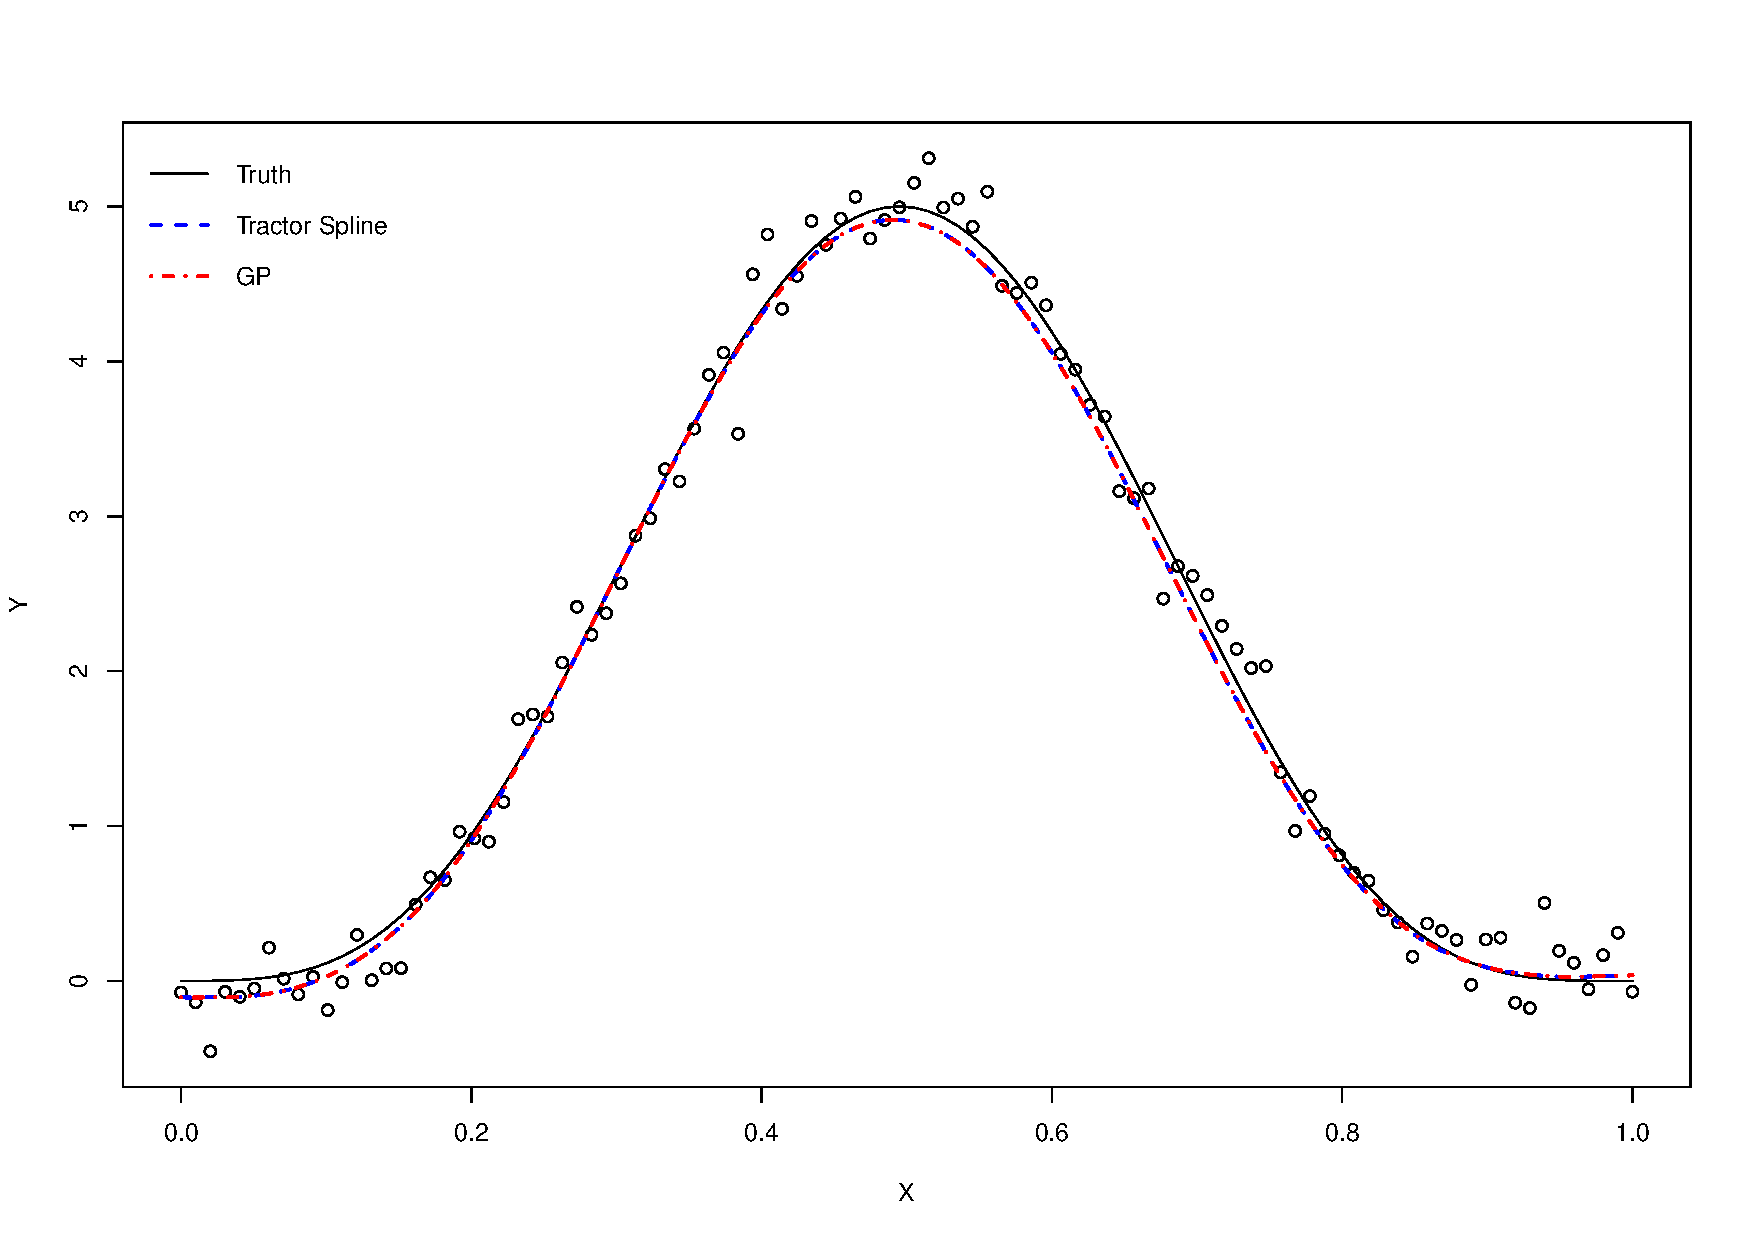
\includegraphics[width=0.8\textwidth]{Chapters/03GPR/plot/sim_cov} 
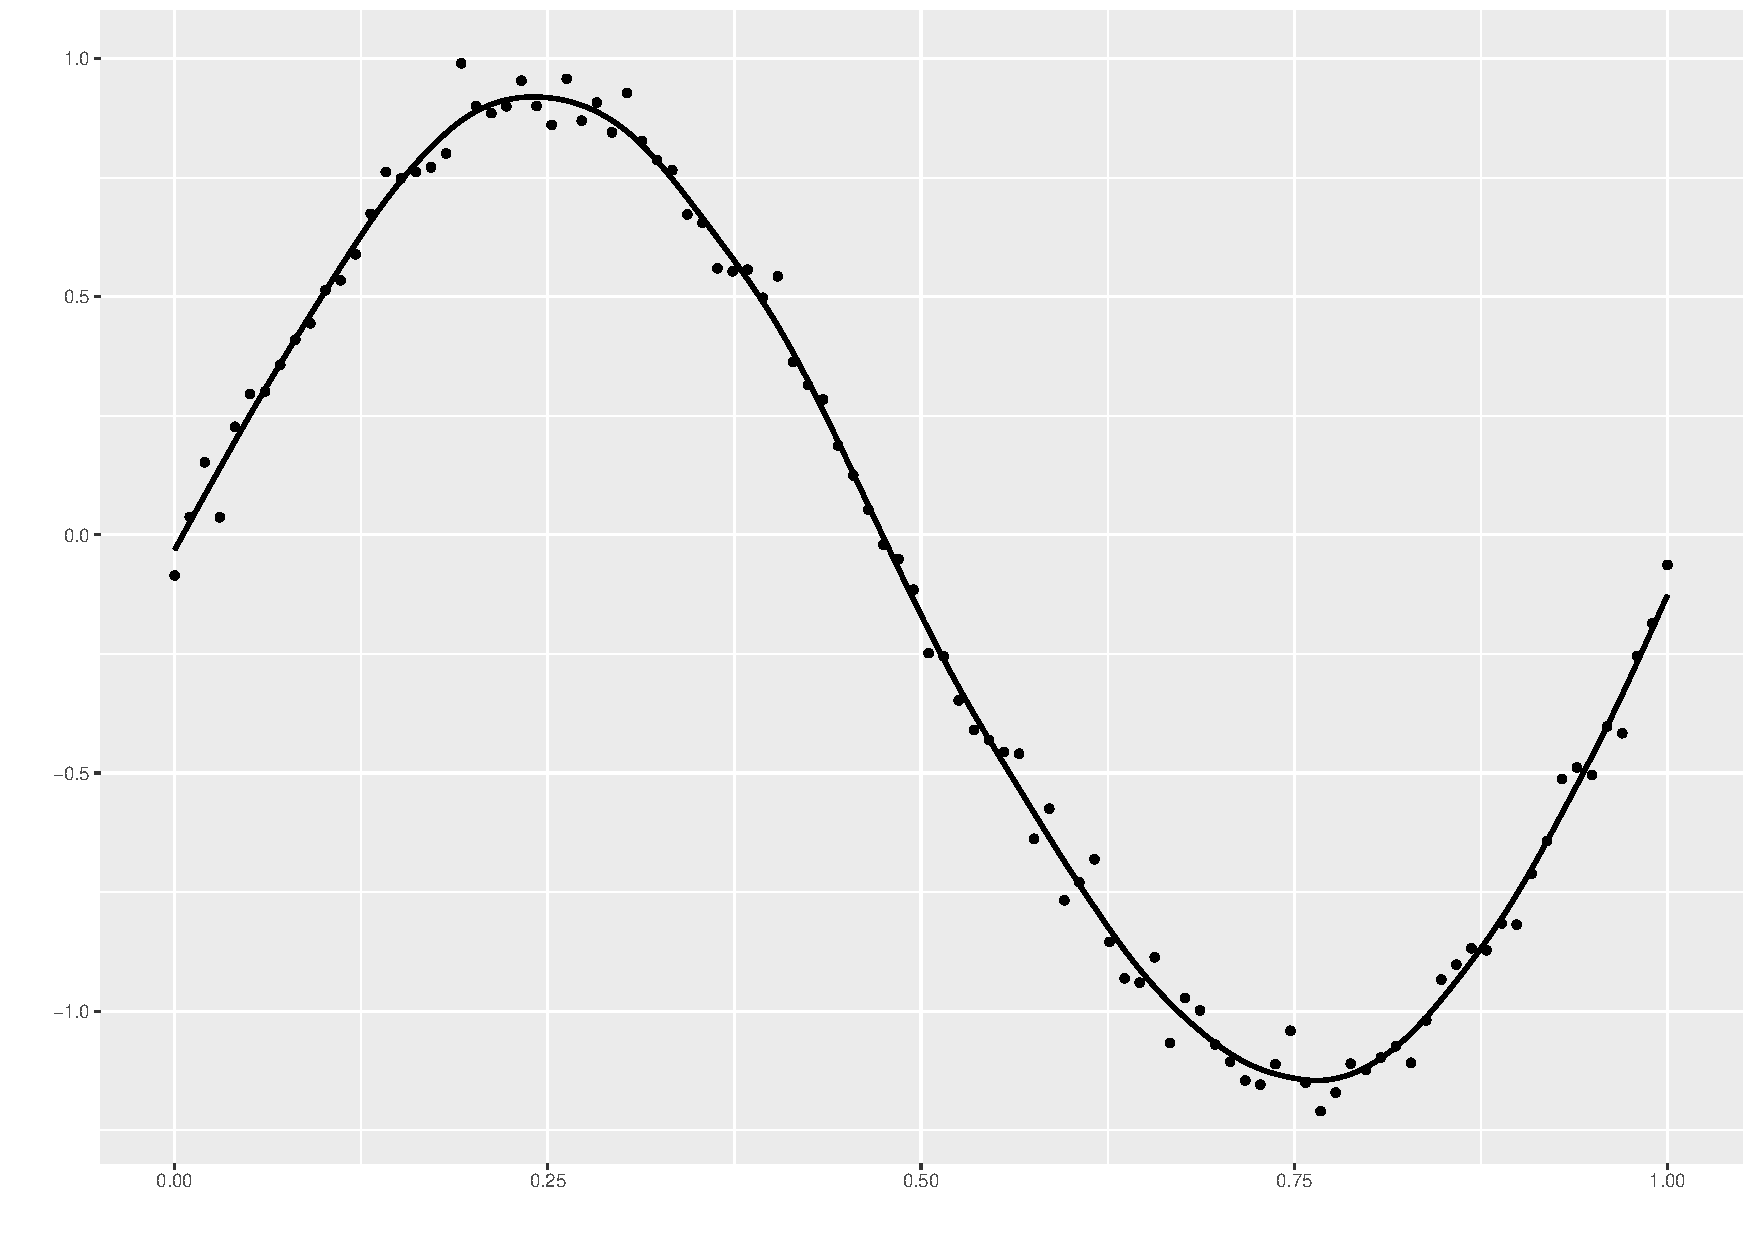
\includegraphics[width=0.8\textwidth,height=8cm]{Chapters/03GPR/plot/ggsim_cov} 
 \caption{Comparing (trivial) Tractor spline and its Bayes estimate. Two methods are corresponding to each other. In this figure, black dots indicate observations and solid line stands for the reconstruction. The Tractor spline and its posterior $\E(f(t) \mid \mathbf{y}, \mathbf{v})$ of Bayes estimate give the same results. }
\end{figure}



\section{Conclusion}

In this Chapter, we take a review on the work have been done in the last few years for the relationship between polynomial smoothing spline and the Bayes estimates. With improper priors, the two methods are corresponding to each other. In fact, smoothing spline is a particular case of Gaussian process regression. By following the work done by \cite{gu2013smoothing}, we find the Bayes estimate for Tractor spline with a constant penalty parameter $\lambda$.  However, it is a particular scenario of Tractor spline whose $\lambda(t)$ varying on domains. So the trivial Tractor spline might not be an optimal solution. Additionally, we give the formula of GCV for Tractor spline with correlated errors on $y$ and $v$. 


A further work is to find the Bayes estimate for the real Tractor spline with a piecewise penalty term $\lambda(t)$. Besides GCV, other methods, such as EM and UBR are worth being invested in further research. 








